\documentclass[a4paper,12pt]{report}

\usepackage[top=2.5cm, bottom=3cm, left=3cm, right=2cm]{geometry}
\usepackage{mathtools}
\usepackage{amsthm}
\usepackage[bitstream-charter]{mathdesign}
\usepackage[pdftex]{graphicx}
\usepackage{fixltx2e}
\usepackage{afterpage}
\usepackage[acronym,nomain]{glossaries}
\usepackage{latexsym}
\usepackage{times}
\usepackage{amsmath}
\usepackage{subfigure}
\usepackage{multirow}
\usepackage{rotating}
\usepackage[table]{xcolor}
\usepackage[acronym,nomain]{glossaries}
\usepackage{setspace}
\usepackage[nottoc]{tocbibind}
\usepackage[toc,page]{appendix}


\newcommand{\HRule}{\rule{\linewidth}{0.5mm}}
\newenvironment{dedication}
  {\clearpage		% we want a new page
   \thispagestyle{empty}% no header and footer
   \vspace*{\stretch{1}}% some space at the top
   \itshape		% the text is in italics
   \centering		% flush to the right margin
  }
  {\par			% end the paragraph
   \vspace{\stretch{3}} % space at bottom is three times that at the top
   \clearpage		% finish off the page
  }

\newtheorem{theorem}{Theorem}
\newtheorem{remark}{Remark}
\newtheorem{definition}{Definition}
\newtheorem{corollary}{Corollary}
\newtheorem{lemma}{Lemma}
\newtheorem{note}{Note}
\makeglossaries

%%%%%%%%%%

\begin{document}

\begin{titlepage}
\begin{center}
\HRule \\[0.4cm]
{\huge \bfseries \textbf{Video Integrity Analysis with BlockChain Technology}  \\[0.4cm] }
\HRule \\[1cm]
\end{center}
\vspace{0.2cm}
\begin{center}
{\large{Bachelor Thesis}}
\end{center}
\vspace{0.25cm}
\begin{center}
{\large {\textsc{By}}}
\end{center}
\vspace{0.35cm}
\begin{center}
{\large{Anuj Kr. Pathak\\Sayan Shankhari}}
\end{center}
\vspace{0.25cm}

\begin{figure}[h]
    \centering
        
\includegraphics[width=0.25\textwidth]{iiitk}
\end{figure}

\vspace{0.5cm}

\begin{center}
{\textit{\Large{A thesis submitted to}}}\\
\end{center}

\vspace{0.25cm}

\begin{center}
{\Large{IIIT Kalyani}}\\
\end{center}

\vspace{0.35cm}

\begin{center}
\textit{\large {for the partial fulfillment of the degree of}}\\
\vspace{0.8cm}
\textbf{\Large{Bachelors of Engineering in Computer Science}}\\
\end{center}

\begin{center}
\textbf{{\large{in}}}
\end{center}

%\vspace{0.1cm}
\begin{center}
\textbf{\Large{Department of Computer Science and Information Technology}}\\
\end{center}

\vspace{0.5cm}
\begin{center}
\Large{December, 2018}
\end{center}
\end{titlepage}

%%%%%%%%%%

\newpage
\chapter*{}
\setcounter{page}{1} \pagenumbering{roman}
\begin{center}
\textbf{\textsc{\Large Certificate}}\\[0.75cm]
\end{center}
\onehalfspacing This is to certify that the thesis entitled
\textbf{Video Integrity Analysis with BlockChain Technology} being submitted by undergraduate students \textbf{Anuj Kr. Pathak} (Id: 000000102) and \textbf{Sayan Shankhari} (Id: 00000121) in the Department of Computer Science and Information Technology, Indian Institute of Information Technology Kalyani, Nodia, 741235, India, for the award of \textbf{Bachelors of Technology} in \textbf{Computer Science \& Engineering}, is an original research work carried by them under my supervision and guidance. The synopsis has fulfilled all the requirements as par the regulation of \textbf{IIIT Kalyani} and in my opinion, has reached the standards needed for submission. The works, techniques and the results presented have not been submitted to any other university or Institute for the award of any other degree or diploma.\\
\bigskip
\bigskip
\bigskip
\bigskip
\bigskip
\bigskip
\bigskip
\begin{flushleft}
\bigskip
(\textbf{Dr. Imon Mukherjee, Ph.D})\\
\smallskip
Assistant Professor\\
Department of Computer Science and Information Systems\\
Indian Institute of Information Technology Kalyani\\
IIIT Kalyani Campus, West Bengal 741235, India.
December 2018\\
\end{flushleft}

%%%%%%%%%%

\newpage
\begin{dedication}
\textit{To my beloved parents and friends who have supported me and prayed for
my success\\ throughout my life.}
\end{dedication}

\chapter*{Acknowledgments}
First of all, We would like to take this opportunity to thank my supervisor Dr. Imon Mukherjee without whose effort this thesis would not have been possible. We are so grateful to him for working tirelessly after us, clearing our doubts whenever and wherever possible. We are most grateful to Department of Computer Science and Information Technology, Indian Institute of Information Technology Kalyani, West Bengal, 741235, India, for providing us this wonderful opportunity to complete our bachelor thesis. We would like to thank our friends for providing us help as and when required. We would like to thank our team mates for being a great motivators and great friends.\\
\\
\linebreak And last but the biggest of all, We want to thank our parents, for always believing in us and letting us do what we wanted, but keeping a continuous check that we never wandered off the track from my goal.\\

\bigskip
\bigskip
\bigskip
\bigskip
\begin{flushleft}
\bigskip
\textbf{Anuj Kr. Pathak}\\
\smallskip
Id. No.: 00000102\\
\bigskip
\bigskip
\bigskip
\textbf{Sayan Shankhari}\\
\smallskip
Id. No.: 00000121\\
\bigskip
December, 2018\\
\end{flushleft}

%%%%%%%%%%

\newpage
\chapter*{Abstract}
A purely peer-to-peer version of online data would allow online transactions to be sent directly from one node to another without going through a central authority. Digital signatures provide part of the solution.
The network timestamps transactions by hashing them into an ongoing chain of hash-based proof-of-work, forming a record that cannot be changed without redoing the proof-of-work. The longest chain not only serves as proof of the sequence of events witnessed, but proof that it came from the largest pool of CPU power. As long as a majority of CPU power is controlled by nodes that are not cooperating to attack the network, they'll generate the longest chain and outpace attackers. The network itself requires minimal structure. Messages are broadcast on a best effort basis, and nodes can leave and rejoin the network at will, accepting the longest proof-of-work chain as proof of what happened while they were gone.
To prevent the action against one of the biggest issues in India of Fake Video Scam. This project tries to find a way to prevent it with a new upcoming technology.

\textbf{Keywords:} Peer-to-Peer network, Proof-of-work, Proof-of-Stake, Distributed Ledger (Hyper-Ledger), Concensus Mechanism, Hash Function, Video Formatting, Video File formats, Watermarking, Android, WebServer.

%%%%%%%%%%

\pagebreak \tableofcontents

%%%%%%%%%%

\afterpage{\null\newpage}

\chapter{Introduction}
\label{Ch1} \setcounter{page}{1} \pagenumbering{arabic}
\bigskip
\bigskip
\bigskip
This chapter presents the introduction of the thesis that includes the brief description of BlockChain, and the adopted approach to address the problems. This chapter also presents the scope of this thesis and the contributions of the thesis.

\section{BlockChain}
A BlockChain can be broadly described as a peer-to-peer network of nodes that makes a collaborative effort in sensing certain specified chain of blocks of data around its periphery and thereby controls the surrounding environment. In BlockChains, each node consists of processing capability, it may contain multiple types of memory like program, data and memories, having a Web-Service transceiver, Client-Server processors, and a power source. The nodes communicate with each other using web-services and self-organized.

\begin{figure}
\begin{center}
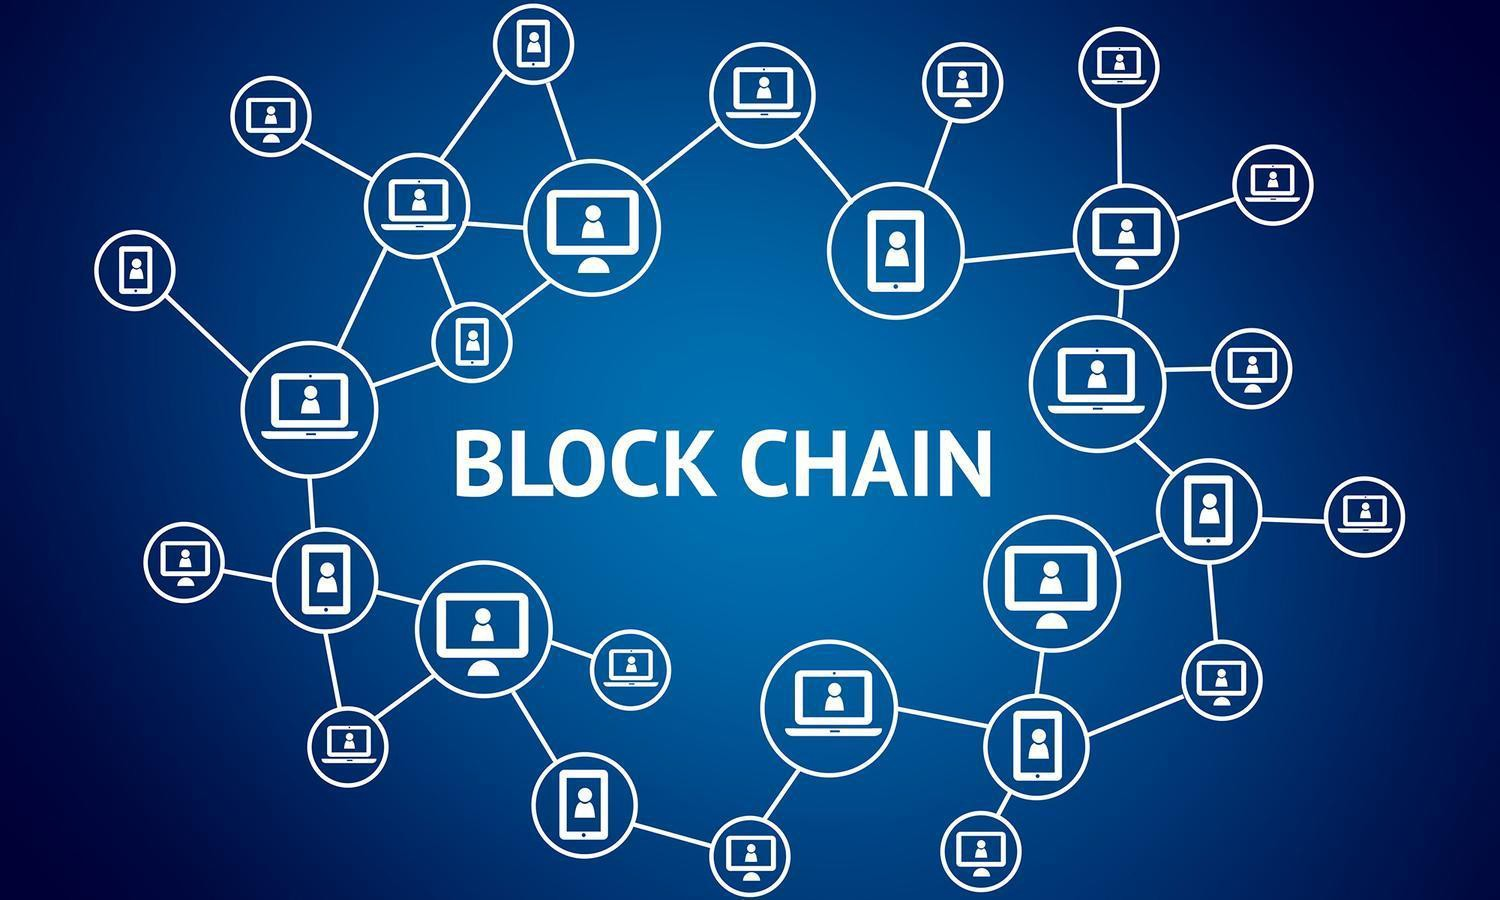
\includegraphics[width=0.8\textwidth]{blockchain.jpeg}
\end{center}
\caption{Overview of Block-Chain Technology (BCTs).}
\end{figure}

\section{Applications of BCTs}
Block-Chain Technology provides one major advantage over conventional centralized database system: immunity from unexpected data changes or Hacks, which gives rise to numerous applications. Some of them include

\begin{itemize}
\item Crypto-currency: Creating and transferring digital money, Data Mining.
\item Military applications: Secure and verified records of Every Military Events and documents.
\item Structural health Monitoring
\item e-Biding Systems
\item Election System or e-Voting Systems
\item Selling Records and other Commercial Applications
\item Music Copyright Verification System
\item Video Message integrity Testing
\end{itemize}

\section{Security and Integrity in BCTs}
As the data is not sitting on a single data server so there is no security issue for Server Hacking. And also the hash-Chain with Cryptography makes it near to impossible to figure out or change previous data block in the blockchain. Before adding any data block with the help of consensus mechanism the blocks are verified with the digital signature of the node and some solution of nonce.

\section{Thesis Contribution}
The main contributions of the thesis includes
\begin{enumerate}
\item Proposes an user anonymity-preserving algorithm to be a part of Video Integrity Program.
\item Formally analyzes the security of the newly designed protocol as well as its performance.
\item The scheme, as compared to the existing schemes, not only authenticates the users but, also establishes a session key between the user and the System after successful mutual authentication.
\item The scheme provides many security and robustness features of user authentication and Block Processing scheme for BCTs.
\end{enumerate}

\section{Roadmap of the Thesis}
The structure of the thesis is as follows:
\begin{enumerate}
\item The Chapter \ref{Ch1} is an introductory part which discusses the scope of the thesis, about the contribution of this thesis and the motivation for writing it.
\item The Chapter \ref{Ch2} provides the background of BCTs, applications of BCTs, security aspects of BCTs.
\item The Chapter \ref{Ch3} discusses in details the basis of ECC, some definitions for security and some mathematically intractable problems.
\item The Chapter \ref{Ch4} introduces the proposed authentication framework after highlighting the motivations behind this work.
\item The implementation of Chapter \ref{Ch5}, where an informal implementation of the proposed protocol has been discussed.
\item The Chapter \ref{Ch6} comprises of the conclusion and further work of the Project in future.
\end{enumerate}

\afterpage{\null\newpage}

%%%%%%%%%%

\chapter{Background}
\label{Ch2} \setcounter{page}{1} \pagenumbering{arabic}
\bigskip
As we all know that in India the politics and the social media is a big thing for people to consider as an important part of life. But the problem is that some social media users does think of exploiting with the content either by downloading the video or recording on screen and uploading it to the social media platforms. Those new videos might be very sensitive and controversial and that becomes viral.
\par What is needed is an digital verification system based on cryptographic proof instead of trust,
allowing any two willing parties to transact directly with each other the video files related information without the need for a trusted third party. Transactions that are computationally impractical to reverse would protect sellers from fraud, and routine escrow mechanisms could easily be implemented to protect buyers. In this paper, we propose a solution to the double-spending problem using a peer-to-peer distributed timestamp server to generate computational proof of the chronological order of transactions. The system is secure as long as honest nodes collectively control more CPU power than any cooperating group of attacker nodes.



\chapter{Details}
\label{Ch3} \setcounter{page}{1} \pagenumbering{arabic}
\bigskip

The process underlying the block-chain technology are the folowing:
\begin{itemize}
\item Creating Account and Be a Part of the Network with an hash id
\item Creating own Data block
\item Request the BCT System to add it by sending it to the open Network in secure or enCrypted way
\item The system then send the block to other nodes for verification
\item The other nodes can verify it with solving some nonce and report to system
\item After being verified the System will add the new block to the chain and update it to every peer's copy of the hyper-ledger
\item Data mining is useful when to check again and again for the integrity of data and the performance of the system
\end{itemize}

The following is the overview of the BitCoin implemention using concepts of blockchain,

\section{Transaction}
We define a block data masked with chain of digital signatures. Each owner transfers the coin to the
next by digitally signing a hash of the previous transaction and the public key of the next owner
and adding these to the end of the coin. A payee can verify the signatures to verify the chain of
ownership.

\section{Timestamp}
The solution we propose begins with a timestamp server. A timestamp server works by taking a
hash of a block of items to be timestamped and widely publishing the hash, such as in a
newspaper or Usenet post [2-5]. The timestamp proves that the data must have existed at the
time, obviously, in order to get into the hash. Each timestamp includes the previous timestamp in
its hash, forming a chain, with each additional timestamp reinforcing the ones before it.

\section{Proof of Work}
To implement a distributed timestamp server on a peer-to-peer basis, we will need to use a proof-
of-work system. The proof-of-work involves scanning for a value that when hashed, such as with SHA-256, the
hash begins with a number of zero bits. The average work required is exponential in the number
of zero bits required and can be verified by executing a single hash.
For our timestamp network, we implement the proof-of-work by incrementing a nonce in the
block until a value is found that gives the block's hash the required zero bits. Once the CPU
effort has been expended to make it satisfy the proof-of-work, the block cannot be changed
without redoing the work. As later blocks are chained after it, the work to change the block
would include redoing all the blocks after it.

\section{Network}
The steps to run the network are as follows:
\begin{enumerate}
\item New transactions are broadcast to all nodes.
\item Each node collects new transactions into a block.
\item Each node works on finding a difficult proof-of-work for its block.
\item When a node finds a proof-of-work, it broadcasts the block to all nodes.
\item Nodes accept the block only if all transactions in it are valid and not already spent.
\item Nodes express their acceptance of the block by working on creating the next block in the chain, using the hash of the accepted block as the previous hash.
\end{enumerate}

\section{Incentive}
By convention, the first transaction in a block is a special transaction (the block is called genesis block) that starts a new block owned
by the creator of the block. This adds an incentive for nodes to support the network, and provides
a way to initially distribute coins into circulation, since there is no central authority to issue them.
The steady addition of a constant of amount of new coins is analogous to gold miners expending
resources to add gold to circulation. In our case, it is CPU time and electricity that is expended.

\section{Claiming Memory}
Once the latest transaction in a coin is buried under enough blocks, the spent transactions before
it can be discarded to save disk space. To facilitate this without breaking the block's hash,
transactions are hashed in a Merkle Tree, with only the root included in the block's hash.
Old blocks can then be compacted by stubbing off branches of the tree. The interior hashes do
not need to be stored.

\section{Simplified Video Verification}
It is possible to verify video without running a full network node. A user only needs to keep
a copy of the block headers of the longest proof-of-work chain, which he/she can get by querying
network nodes until he's/she's convinced he/she has the longest chain, and obtain the Merkle branch
linking the transaction to the block it's timestamped in. He can't check the transaction for
himself, but by linking it to a place in the chain, he can see that a network node has accepted it,
and blocks added after it further confirm the network has accepted it.

\section{Privacy}
The traditional banking model achieves a level of privacy by limiting access to information to the
parties involved and the trusted third party. The necessity to announce all transactions publicly
precludes this method, but privacy can still be maintained by breaking the flow of information in
another place: by keeping public keys anonymous. The public can see that someone is sending
an amount to someone else, but without information linking the transaction to anyone. This is
similar to the level of information released by stock exchanges, where the time and size of
individual trades, the "tape", is made public, but without telling who the parties were.

\chapter{Proposal}
\label{Ch4} \setcounter{page}{1} \pagenumbering{arabic}
\bigskip

Using the concepts of Block-Chain we propose our algoorithms for Video Integrity Analysis D-APP system.

We are trying to build a Mobile social media application like WhatsApp and that will be connected with the online server running blockchain in it. The process of verification of the media (text, image or video) for checking fakeness or scam in a nutshell will be as follows,

\begin{itemize}
\item User logs into the account with hashed id
\item User shares media into the social platform by capturing or texting
\item System checks for match with previous hash if the content is already present in the network
\item System stores the data as a block into the blockchain, along with creating the cryptographic hashes
\item User sends video for verification
\item System hashes it and looks into the blocks for same video
\item If found, System decodes the file and search for the metadata containing the source and Watermarks
\item System process the result
\item System publishes the expected result
\item User finds it in his/her mobile client app
\end{itemize}


\chapter{Implementation}
\label{Ch5} \setcounter{page}{1} \pagenumbering{arabic}
\bigskip

The setup we have is like this:
Computer Name: Lenovo \\
Computer OS: Ubuntu 16.04 LTS \\
Runtime Platform: Java 1.0.0\_131 \\

We have tried to make basic blockchain platform without video processing right now. The screenshot of the process is the following,
\begin{figure}[!htb]
\center{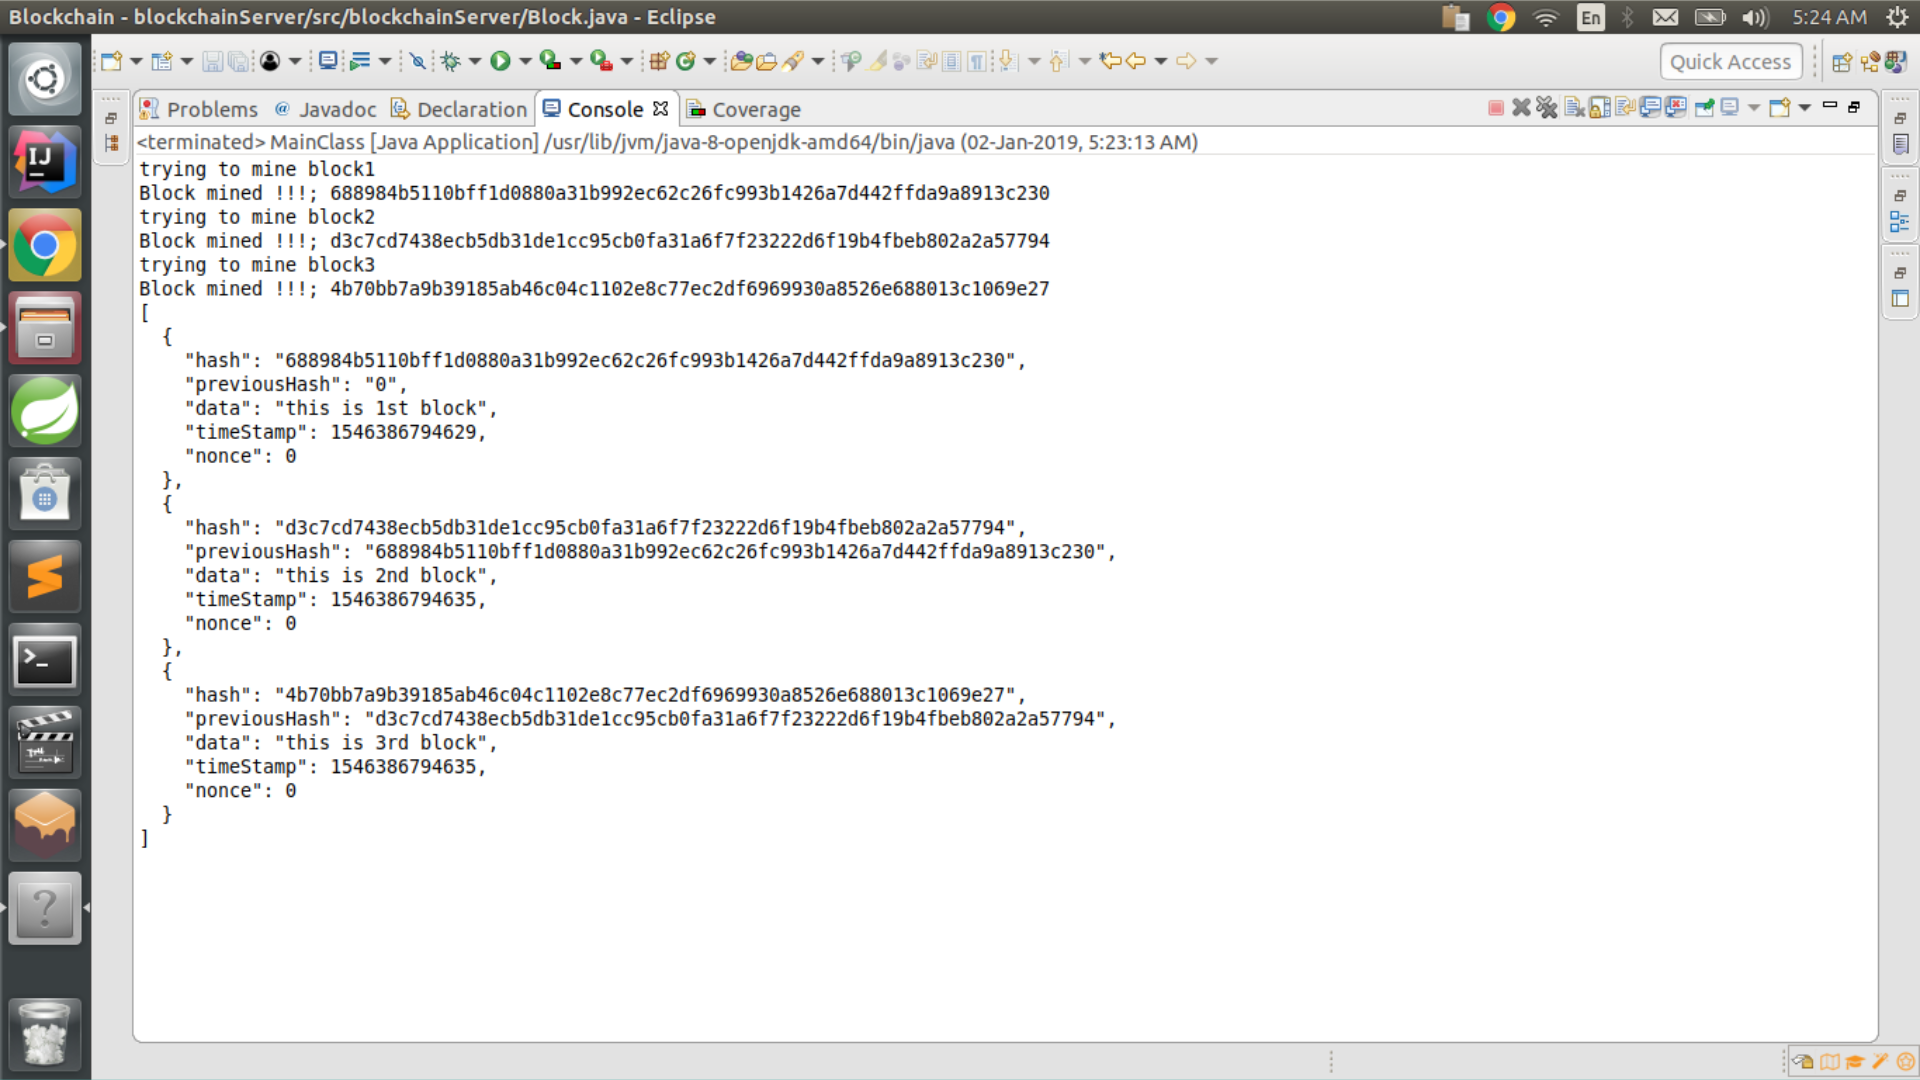
\includegraphics[width=\textwidth]{p0.png}}
\caption{\label{fig:my-label}. Implementation Runtime in Terminal}
\end{figure}
This picture shows how we have created the basic blockchain platform with the following java tools:
\begin{itemize}
\item Image API
\item SHA-256 API
\end{itemize}
There is a very simple concensus mechanism we have used to create the temporary (as the blocks are created and destroyed in the logical memory by Computer Program) private (as right now it is residing in our computer, not in a web server) ledger.\\

As we are implementing in Java, there are publicly functioning classes along with a class containing main function.\\
The classes we have are:\\
	Block\\
	Transaction\\
	String Utility\\
	Main\\

The String Utility contains some manipulation with the SHA-256 program, implemented by Java.\\

The Block contains the following:
Id, 
Timestamp, 
Data, 
Prev hash, 
Nonce\\

For containing the hashes we are using List datatype in Java. Before adding any block we are checking 3 things, that are:\\
Timestamp: The time that it has been created\\
Previous Hash: parent for current block\\
Nonce: Consensus mechanism\\

while using CreateBlock() and MineBlock()

In the transaction class we have,
	Source Name (Hash): transaction from\\
	Destination Name (Hash): transaction to\\

From main, we are
	creating transactions: calling Transaction class
	visiting transactions: receiving hashes


We have planned to include online platform the following way,
\begin{figure}[!htb]
\center{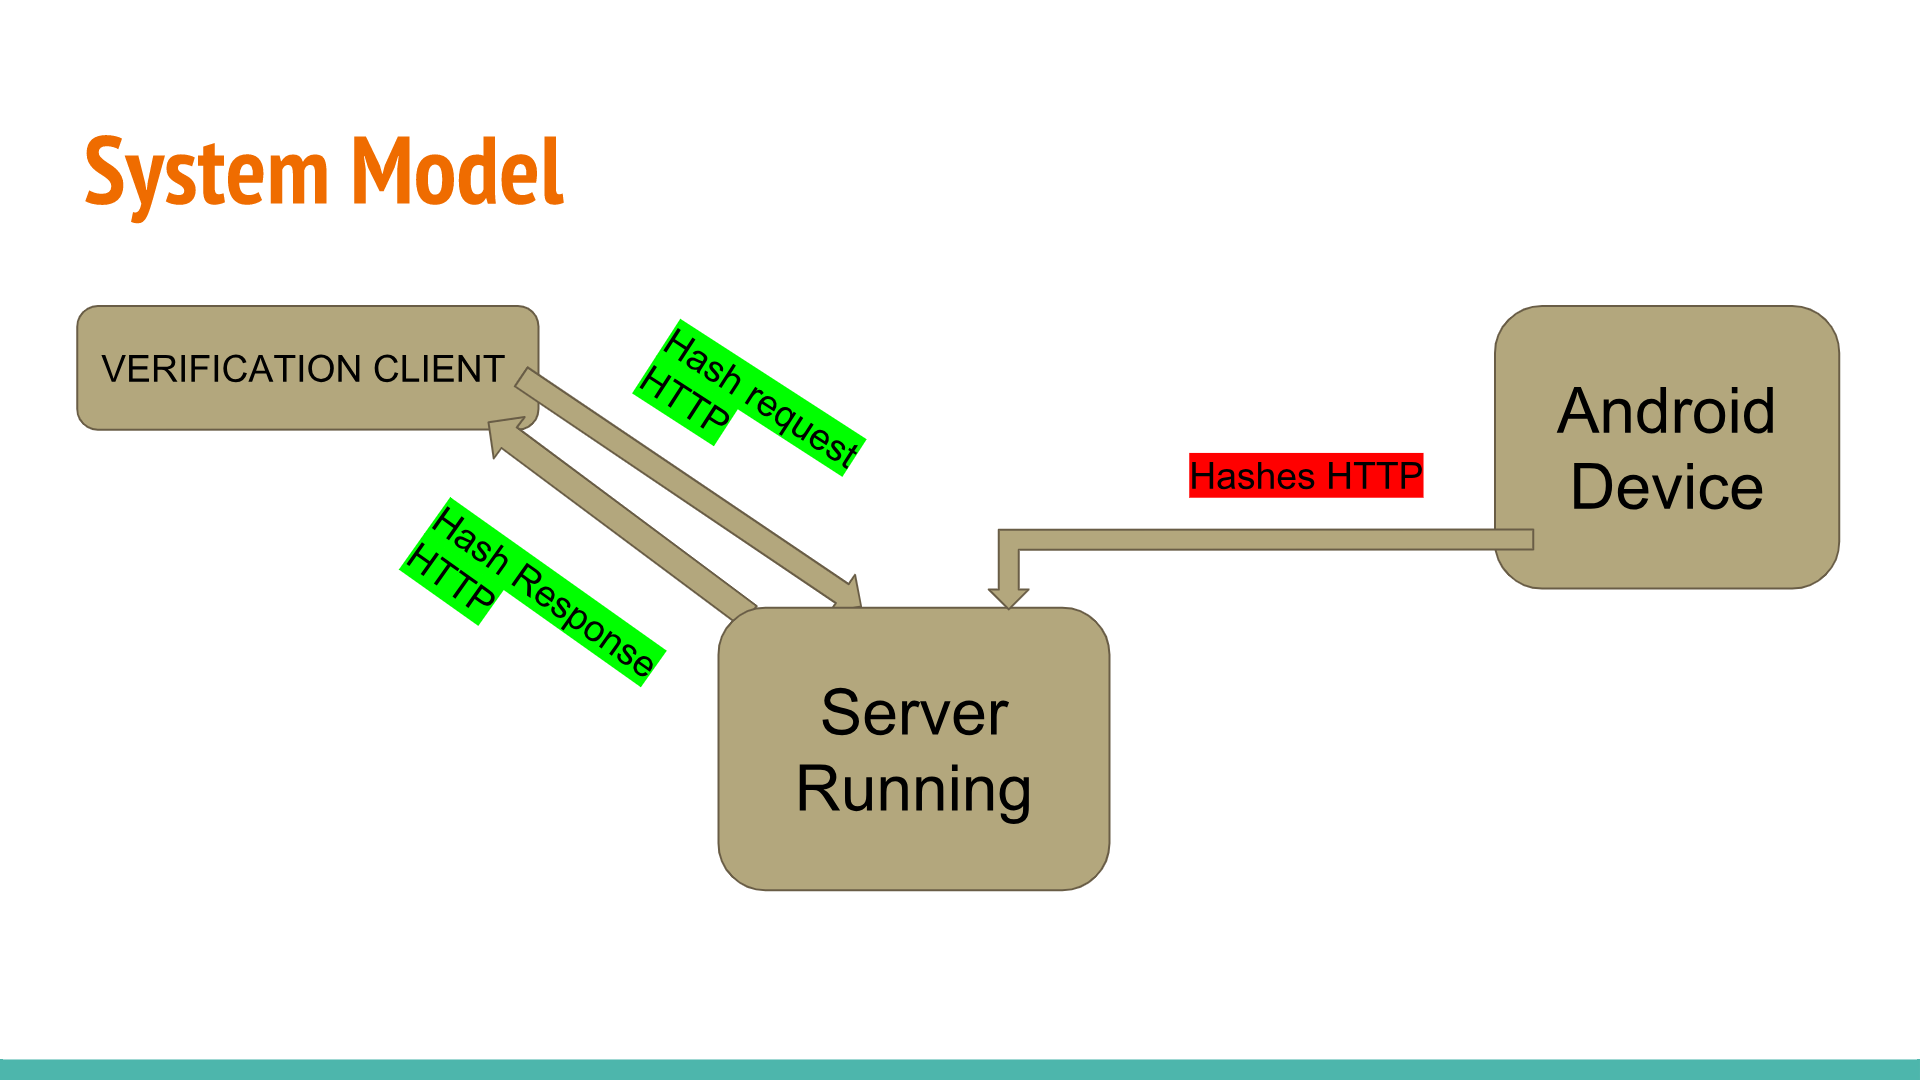
\includegraphics[width=\textwidth]{p1.png}}
\caption{\label{fig:my-label}. System Model}
\end{figure}
In this model we are suggesting that there should be client-server system before involving into the blockchain system. So user have to login first with the hashed id and password. Then the person can apply for either Storing data into system or verify data from the system. The Server will perform the task.\\
\begin{figure}[!htb]
\center{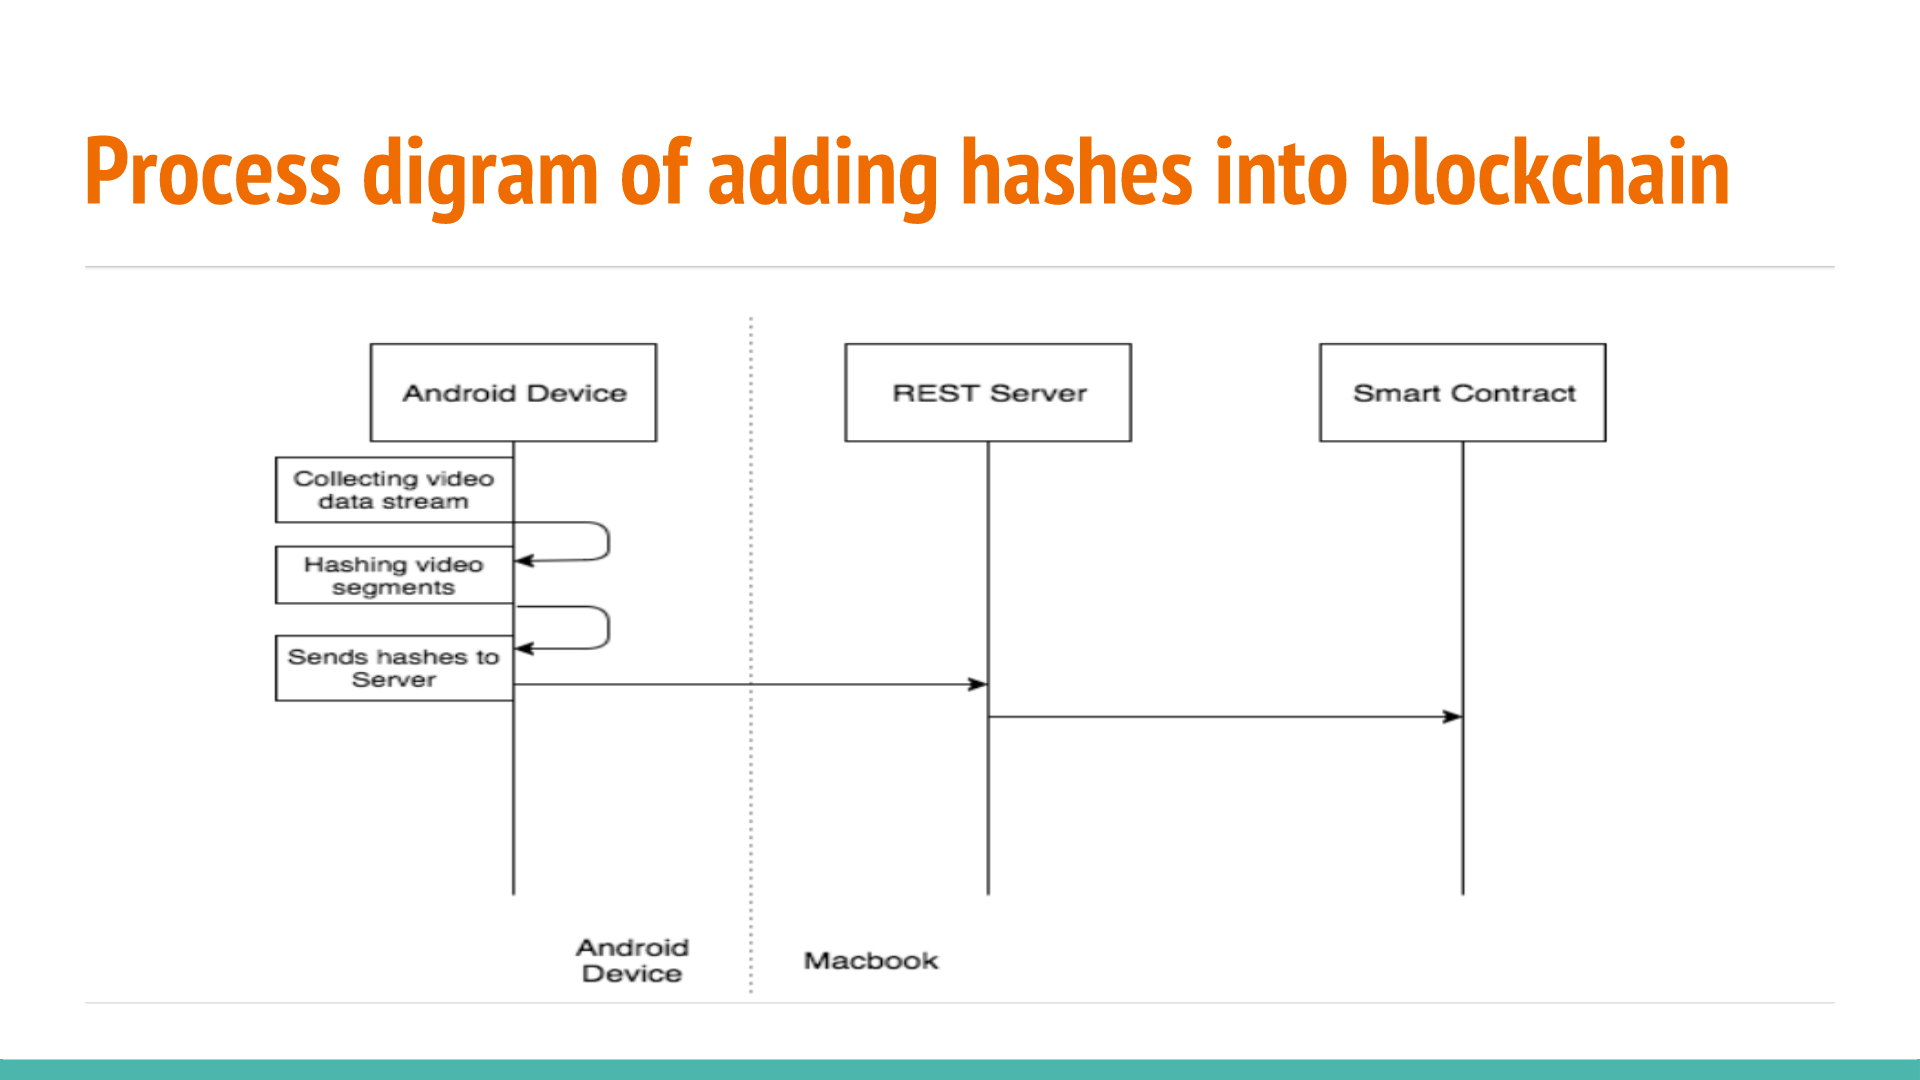
\includegraphics[width=\textwidth]{p2.png}}
\caption{\label{fig:my-label}. Process Diagram with Hashes}
\end{figure}
\begin{figure}[!htb]
\center{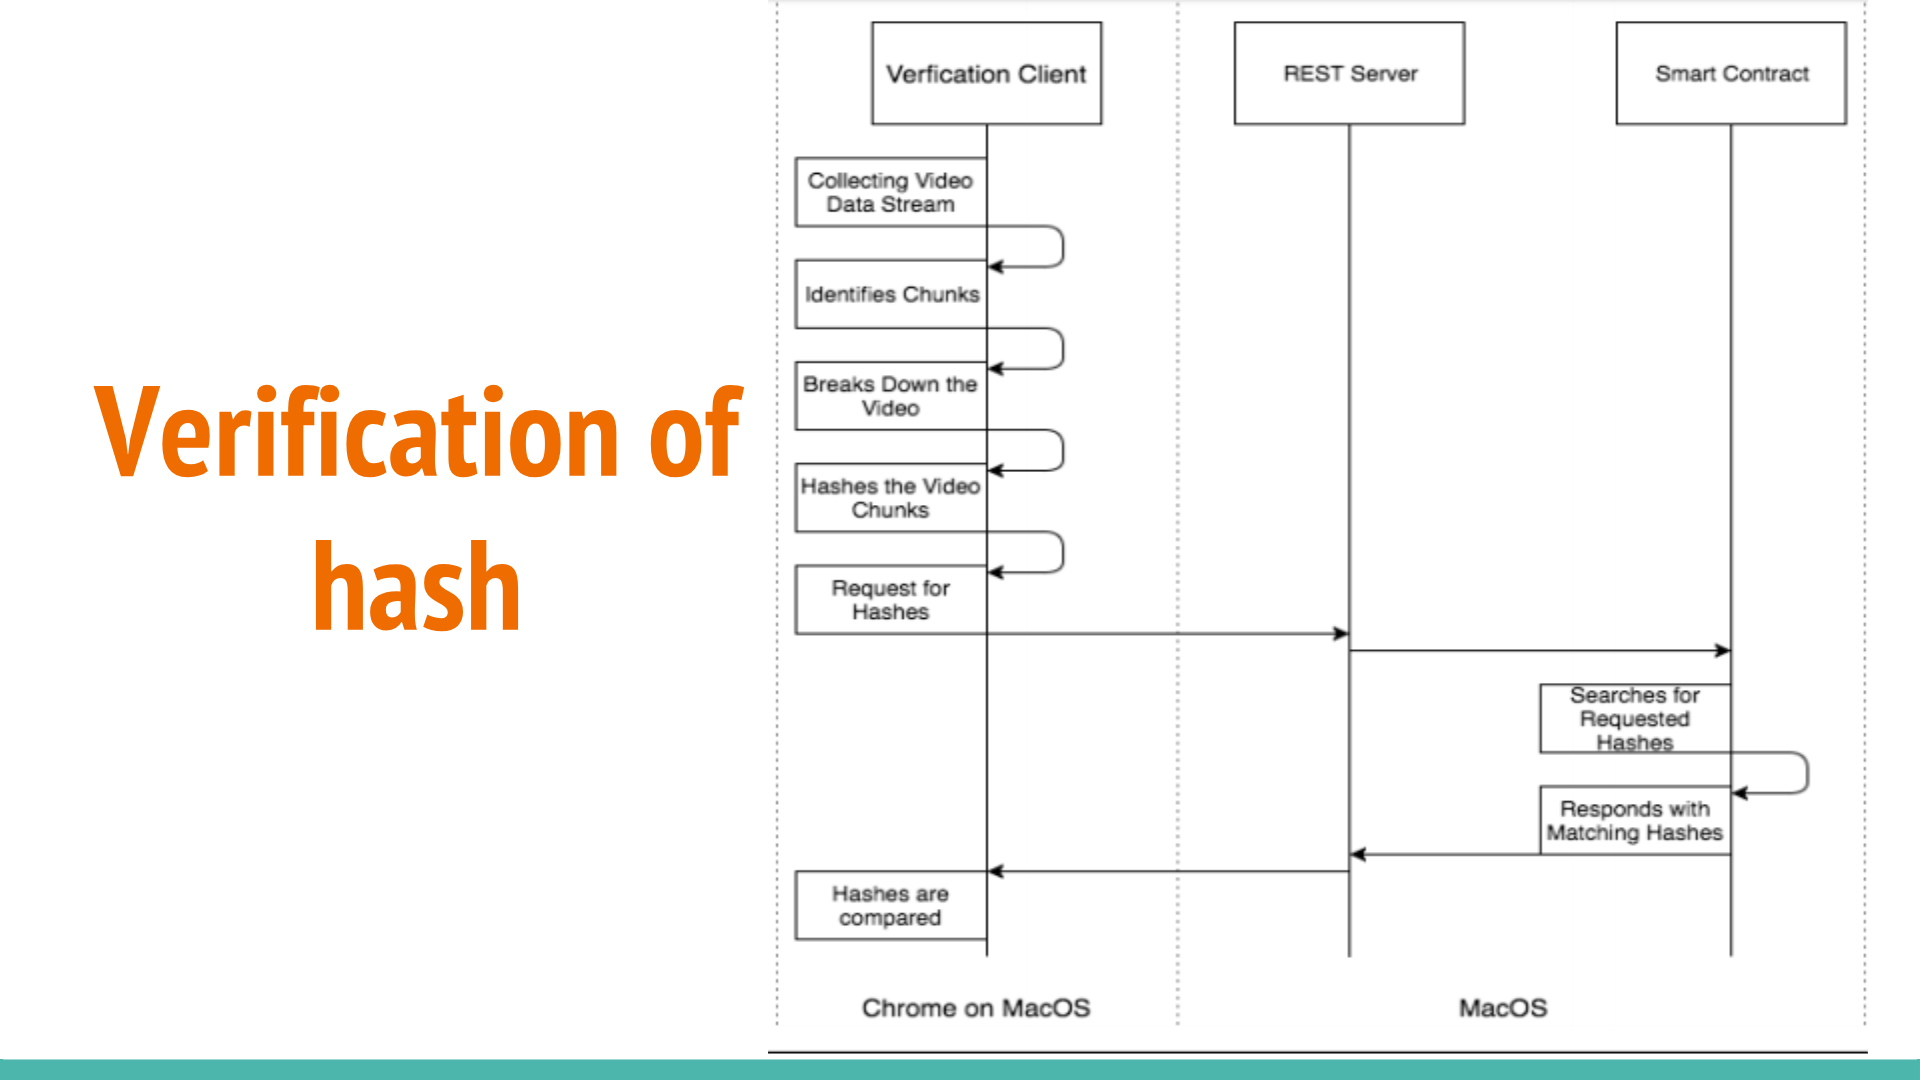
\includegraphics[width=\textwidth]{p3.png}}
\caption{\label{fig:my-label}. Verification Hash}
\end{figure}

\afterpage{\null\newpage}

\chapter{Conclusion and Further Work}
\label{Ch6} This synopsis provides a detailed description of an
Practical implementation of Online Biding system which provides
User Anonymity and Secure Key Exchange and agreement.

\subsubsection{Further Work}
The next target is to make,
\begin{itemize}
\item a software for android that will standalone perform the following tasks
\begin{itemize}
\item Capturing the image or video
\item Processing the video
\item Signing into video
\item Connect to Online Verifier service
\item Send and Receive messages containing Text, Image or Video
\end{itemize}
\item along with the Online Verification Service which will
\begin{itemize}
\item Connect to android app on request
\item Take data, verify and publish result
\end{itemize}
\end{itemize}

\chapter{Bibliography}
We are very thankful to the following contents with their creators which definitely helps to grow our project,
\begin{itemize}
\item Official Site: https://www.blockchain.com/
\item Wiki: https://en.wikipedia.org/wiki/Blockchain
\item Inspired by: "Video Integrity through Blockchain Technology" -by ADAM HEMLIN BILLSTRÖM and FABIAN HUSS
\item Inspired by: "Bitcoin: A Peer-to-Peer Electronic Cash System" -by Satoshi Nakamoto (The Inventor of BlockChain and BitCoin)
\end{itemize}

\end{document}
